\documentclass[a4paper,12pt]{article}
\usepackage[ngerman]{babel}
\usepackage[utf8]{inputenc}

\usepackage{amsbsy,amsmath,amsthm,amssymb}
\usepackage{amsfonts,enumerate}
\usepackage{verbatim,color}
\usepackage{graphicx}
\usepackage{enumitem}
\usepackage{url}

%\setlength{\oddsidemargin}{-1.cm}
%\setlength{\evensidemargin}{-1.cm}
%\setlength{\textheight}{23.5cm}
%\setlength{\textwidth}{16cm}

\setlength{\topmargin}{-1cm}
\setlength{\textheight}{22.5cm}
\setlength{\textwidth}{16cm}
\setlength{\oddsidemargin}{0cm}
\setlength{\evensidemargin}{0cm}
\setlength{\parindent}{0pt}

\newcommand{\RR}{{\mathbb R}}
\newcommand{\code}{\texttt}

\headsep = 0pt
\textheight = 700pt

\begin{document}
\begin{titlepage}
\centering
\vspace*{5cm}

 \includegraphics[width = 1\textwidth]{LEDtrix_Logo.png}
\vspace{1cm}

\large{Computer Architecture and Operating Systems\\Fall semester 2018}
\end{titlepage}
 
 \section{Introduction}
 
 The LEDtrix is a square LED's matrix inside a box made of wood, connected to RaspberryPi as well as to buttons, to play some games on.
 Our aim is to have at least two games, and code which is expandable so one may easily add a new game.
 The problem will be to efficiently calculate the game-logic, whilst updating the LED's continuously.
 If we do not get this right, the LED's will flicker and therefor worsen the gaming experience.
 
 This may lead to more flickering, consequently we have to look for a good solution.
 
\textbf{Introduction to the topic with a problem statement and questions to examine}
 
 \section{Background}
 
 The idea for our project came by coffee tables containing a LED's Matrix.
 We liked this and thought of a way to produce something similar, but easier to transport.
 It needed to be robust for which reason we came up with the idea of a wooden box.
 Then, we needed make up our mind about how to control the games.
 We thought about touch pads, but left this idea go very quickly, seeing as we want to create a vintage feeling.
 This is when we came up with the idea of two buttons.
 This way, we could keep the game logic very simple and concentrate on the more important and interesting parts of our project.
 
 Seeing as we both had no experience with soldering, especially as it would have taken all of the available project time, we decided on using LED-strips instead of 225 separate LED's, which were also less expensive.
 We took the APA-102 strips because they have a clock included.
 It would have been impossible to program this on the RaspberryPi.
 
 \textbf{Introduce and compare relevant technologies, protocols,
algorithms,..}

\section{Building the Box}
We began by building the box, continued by fixating the LED strips and soldering them together.
 Our first problems arouse, when we tried to splice the wooden parts of our box.
 We went to the switch gear workshop of the Elektrizitäts AG Basel to do so, where we realised that this would be very unstable.
 The employees helped us to build the box stronger, by screwing the pieces together, instead of using glue.
 The pictures below show one of the employees helping us to saw the wood (left), and one of us drilling a screw hole into a metal plate, which belongs into one of the corners of the box (right).
 
\vspace{1cm}

{ \centering
  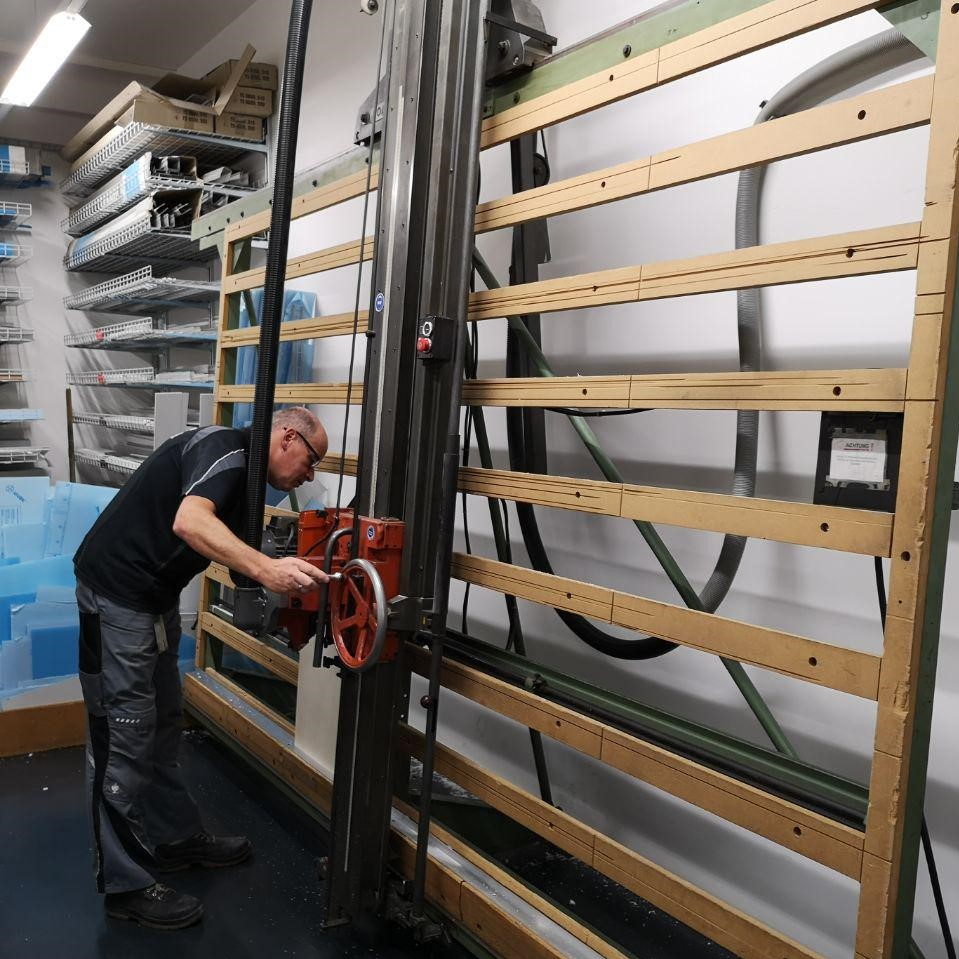
\includegraphics[width = 0.4\textwidth]{brice.jpg}
  \space{   }
  
\includegraphics[width = 0.4\textwidth]{bohren.jpg}
  \\}
 \vspace{1cm}
 
After one day of handicraft work our box was finished, and we ended the day by spraying the outer-wall bright red, what you can see on the picture below (left).
 So the next thing we had to do was to stick the strips onto a wooden board, which you can see us doing so on the picture on the right.
 
 \vspace{1cm}

{ \centering
  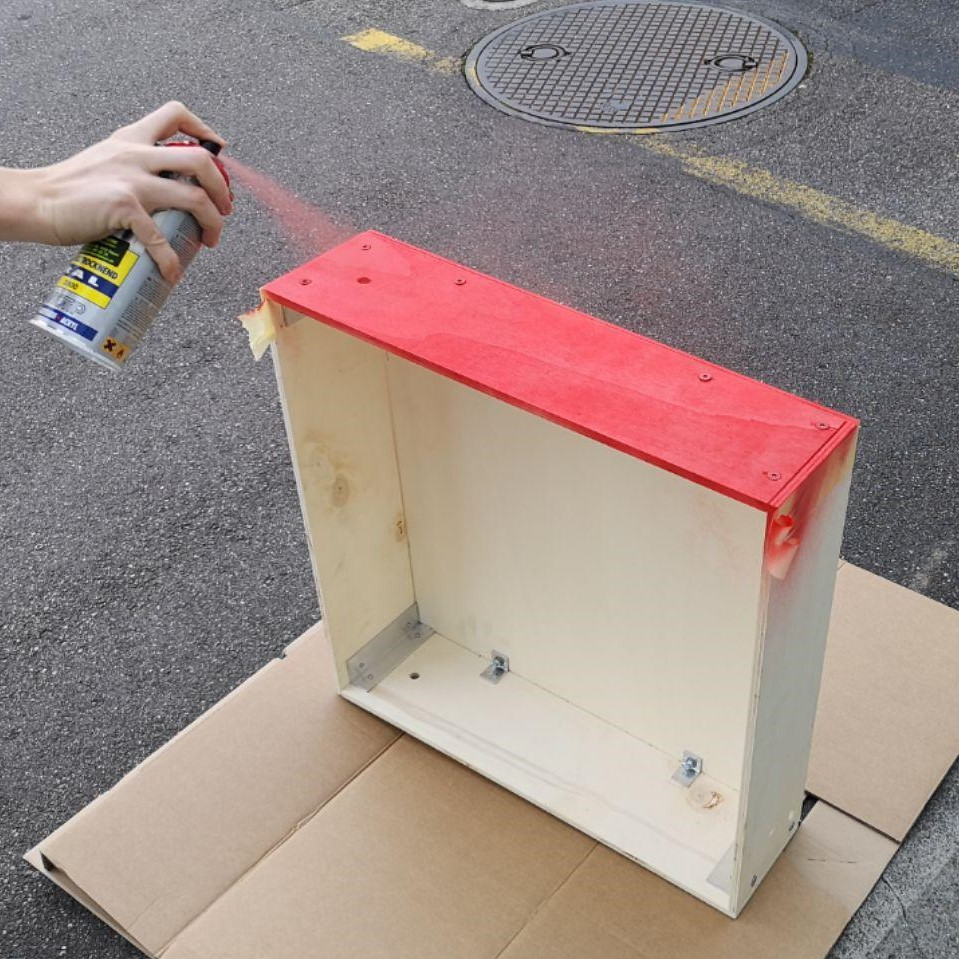
\includegraphics[width = 0.4\textwidth]{sprayen.jpg}
  \space{   }
  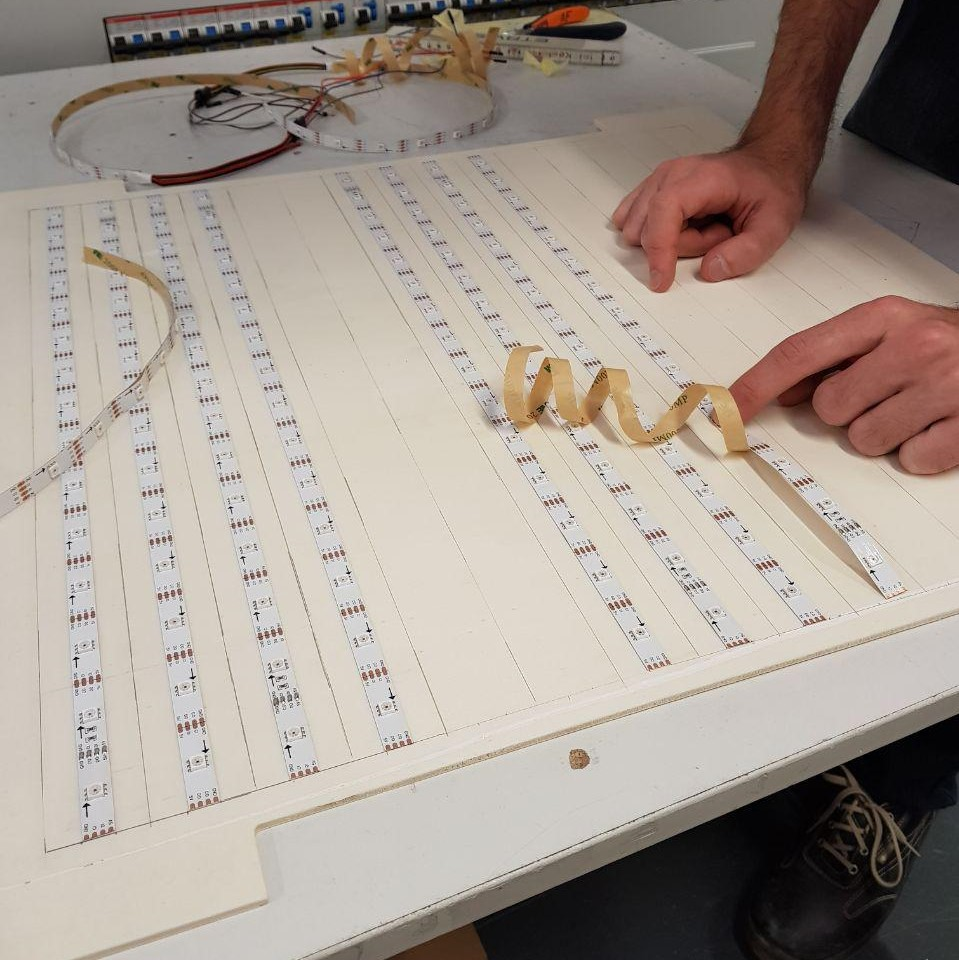
\includegraphics[width = 0.4\textwidth]{kleben.jpg}
  \\}
 \vspace{1cm}
 
After that we had to solder the strips together.
 Since none of us had any experience with soldering, we were surprised how nice it looked and that all of the LED strips were connected and working correctly after the first try.
 Below you see a picture of one of us soldering (left), and the finished LED's board.
 In the beginning we thought about glueing some paper walls between the LED's board and the acrylic glass above it, so we'd have a square for each LED.
 But when we tried it, we both felt it looked nicer without the paper walls, and with no space between the board and the glass, so we did not do that.
 
 \vspace{1cm}

{ \centering
  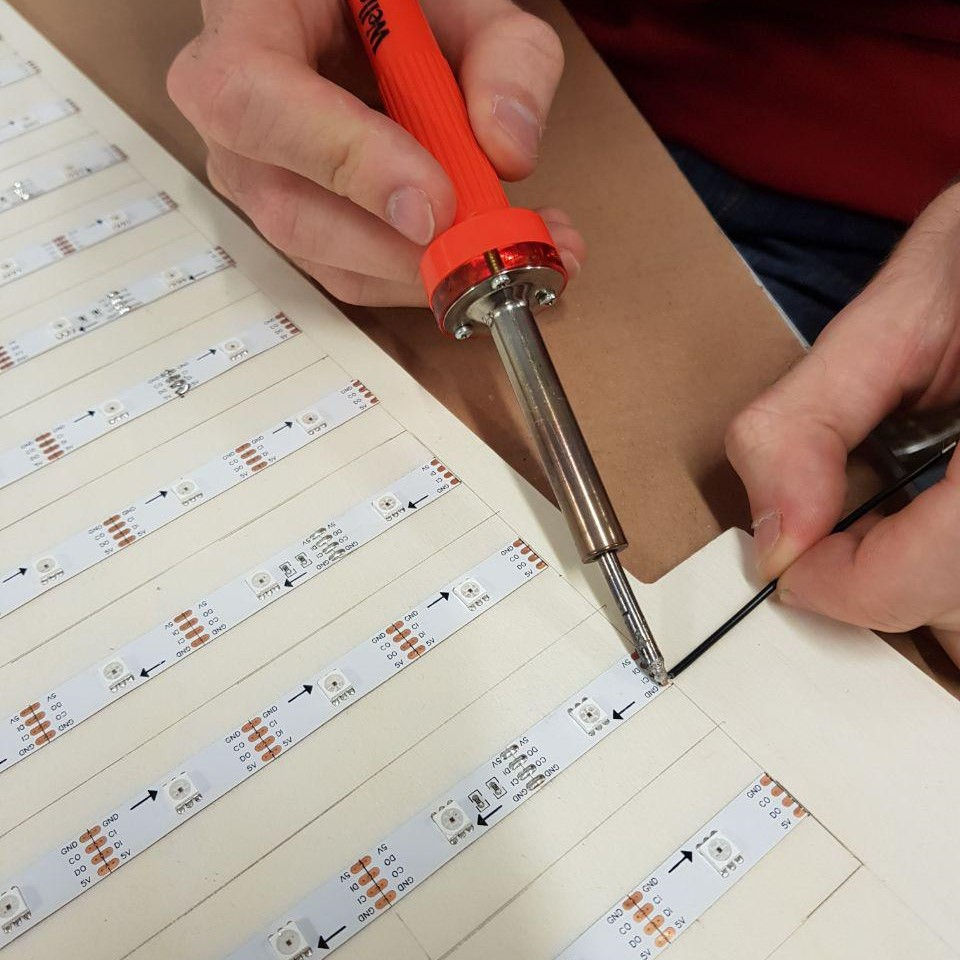
\includegraphics[width = 0.4\textwidth]{loten.jpg}
  \space{   }
  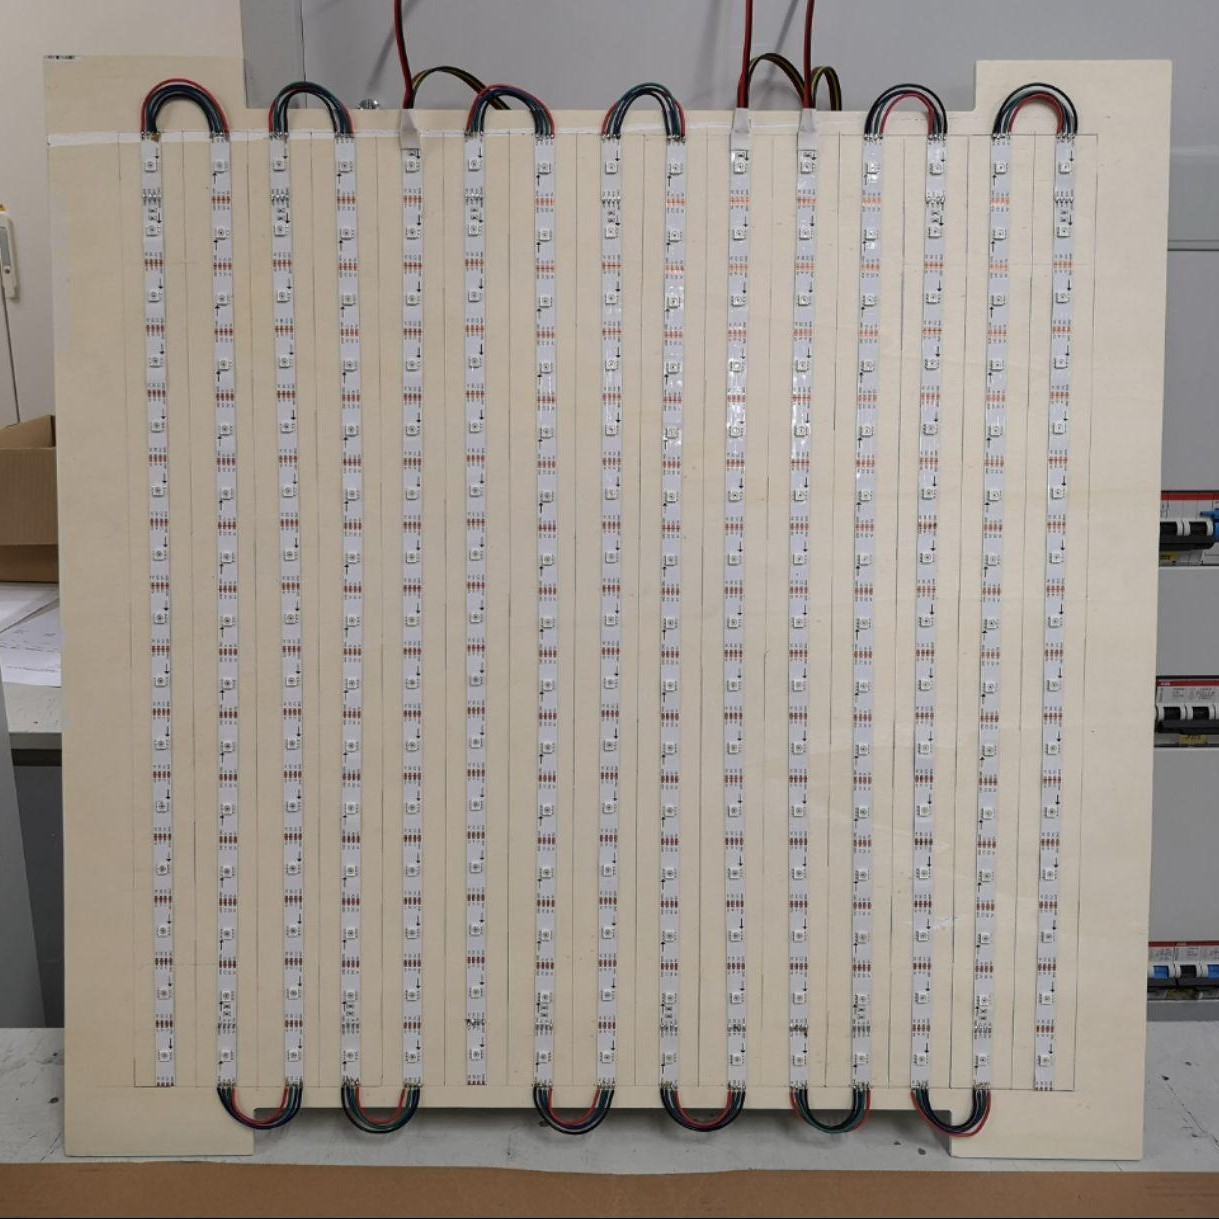
\includegraphics[width = 0.4\textwidth]{matrix.jpg}
  \\}
 \vspace{1cm}
 
\section{Coding}
Before we built the box, both of us started to try different things on the LED's.
 We needed to know how exactly they work and what information we needed to send to display information correctly.
 This could have been very difficult and time consuming, but luckily we came to the correct conclusions really fast.
 We also learned that  the LED's needed so much energy, that we could only have twelve of them blinking at once.
 For this reason we have three blocks of each five strips instead of just one big block.
 
 Another reason for splitting it up, was that 7.5 meters were too long to transport the data efficiently.
 In each of the blocks four LED's are flickering at once, so first the first four, the the next four and so on.
 This happens very fast, for this reason it looks like all of the 225 LED's would be shining at once.
 The first result we had was very disappointing, as the LED's flickered very much, and the colors were inconsistent.
 By spending some time working on it, we made our code more and more efficient, which led to the satisfying result we now have.
 One big change was replacing the wiringPi library with direct memory access, therefore the data could be passed to the strips with less overhead.

After the hardware part was finished, we started programming a demo and each of us a game.
 Since we had no working buttons yet, both of the games had a demo mode which was showed on the LED's.

We thought that with this done, and only the buttons left, the biggest part of the project would have been done.
 But in fact, it was not.
 Our buttons are very imprecise, in fact one click triggers multiple interrupts.
 This is an unusable behavior, as for example while playing Raindrops, one might only go one step to the left and dies, if one push leads to three steps.
 to avoid this, we introduced a timer minimizing the amount of clicks to respond to during a certain interval.
 
 Besides, depending on where in the gaming process one is, we need to react very differently to the buttons being pressed.
 \textbf{We solved this by having Boolean values for both buttons, so when a button is pushed, the Boolean is set to true, and after the information is used, it is set to false.
 Consequently, we are able to react on the push not by complex switch cases in the button handler, but wherever in the code they are needed.}
 
 
 
\textbf{Implementation, Configuration and Setup (conceptional, no description
on code-level and no code)}

\section{Results}
\textbf{Graphics, tables, comparisons, insights..}

\section{Conclusion}
First of all, we are happy our project idea could be accomplished.
 The games are fun to play and look nice, with almost no flickering anymore.

We developed in the Code-and-Fix model, for this reason we had a lot of refactoring, and trying things which didn't work.
 If we would have made some brainstorming in the beginning, probably we would have found a more generic solution.
 
 In addition, due to both of use writing one game and not talking about the structure before, they were not similar.
 When we joined them and the LED's, we had to refactor a lot of things to have inherent code.

Furthermore we should gave taken some notes about decisions and important bugs we removed during the process, since we forgot about some of them.
 When starting the report, we had to think a lot about what we made and why, so we could write it down, which took a lot of time.

\textbf{Discussion/Conclusion/Lessons learned}

\section{References}


\end{document}